% !TEX root = ../thesis.tex

\chapter{Introduction}
\label{chp:intro}

\begin{quotation}
	If you want your figures to look good, generate them to be the exact size that
	they'll be in the final PDF---often measured in points (or inches).  For example, set the width to whatever you provide to \verb|\includegraphis[width=XX]{...}|.  In addition, set the font family and size to match.  Here are reference values:

	\textbf{Full width images:}
	\verb|\textwidth| \the\textwidth{}

	\textbf{Font sizes:}

	\makeatletter
	{\scriptsize \verb|\scriptsize|  \f@size{}pt}

	{\footnotesize \verb|\footnotesize| \f@size{}pt}

	{\small \verb|\small| \f@size{}pt}

	{\normalsize \verb|\normalsize| \f@size{}pt} \textit{\textbf{$\leftarrow$	The size of body and caption text}}

	{\large \verb|\large| \f@size{}pt}

	{\Huge \verb|\Huge| \f@size{}pt}
	\makeatother

	\textbf{Font family:}
	\makeatletter
	\f@family
	\makeatother

	The font family probably reads ``cmr'', which stands for Computer Modern Roman, which is the default font in \LaTeX.  You may be able to download this font and use it in other software when generating figures.  Better yet, when using Python, \href{https://matplotlib.org/stable/users/explain/text/usetex.html}{instruct matplotlib} to render all text using \LaTeX{}.

\end{quotation}

This sample document illustrates how to use the \texttt{thesis} class, originally
written by John P. Weiss.  Some requirements of the Graduate School are written
into that file; page size, line spacing, appropriate placement of captions for
tables and figures, etc.  Revisions by Hongcheng Ni make it possible to use the
(optional) \verb|\usepackage{hyperref}| command to enable internal hyperlinks in
the final PDF document.  The latest version, by Giaco Corsiglia, includes
various other improvements---and has updated this sample file.
Footnotes and references work as follows.  The work presented
here\footnote{Footnotes are handled neatly by \LaTeX.} is an extension of
Lao~\cite{lao:thesis} and Lao et~al.~\cite{lao:paper}, fictional references that
are in the bibliographic source file \texttt{bibliography.bib}.  You should type
citations like this: \texttt{word\textasciitilde}\verb|\cite{ref}|.  Include the
tilde character instead of a normal space so that the bracketed reference
doesn't awkwardly wrap onto a new line.

Figures work well, too.  \Cref{fig:cyl} shows an image from a PDF file
imported into this document using the \verb|graphicx| package.  The command
\verb2\usepackage{graphicx}2, which appears near the very top of the main
\LaTeX{} file, reads in this package which defines the \verb2\includegraphics{}2
macro.  See \cref{fig:drawing} for an example with sub-figures.

Notice the use of the \verb|\cref{...}| commands in the previous paragraph.  This is an enhanced version of the \verb|\ref{...}| command that allows you to avoid typing ``Figure...'' or ``Equation...'' everywhere.  Check out the documentation \href{https://ctan.math.utah.edu/ctan/tex-archive/macros/latex/contrib/cleveref/cleveref.pdf}{here}.

% The letters in the square brackets are hints to LaTeX about where it should place your figures.
% Whether they actually do anything seems pretty random.
\begin{figure}[htbp]
	% Move the caption command here if you want it to display above your figure instead of below.

	\centering
	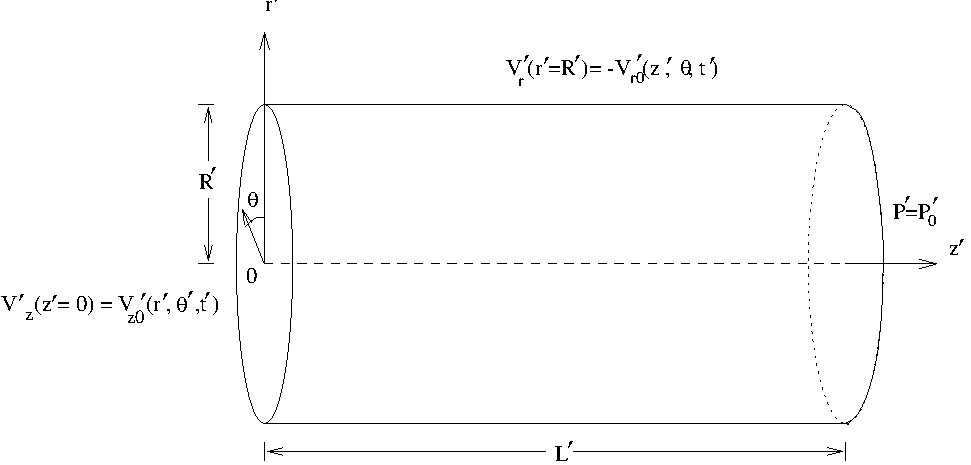
\includegraphics[width=100mm]{chapter-1/cyl.pdf}

	\caption[Cylinder and measurements]{
		Look ma, a figure!  This is the extended caption---but the short version of the caption provided in square brackets will be used in the list of figures at the start of the thesis.  This caption is displayed below the figure.
	}
	\label{fig:cyl}
\end{figure}

\begin{figure}[htbp]
	\centering

  \caption[Figure with sub-figures]{
		This caption is above the figure.  This figure has sub-figures!  Notice in the source that each sub-figure has its own \texttt{label} so that each can be referenced independently.
	}

	\subfloat[JPEG version. You should never use the JPEG format unless you're including an actual photograph.]{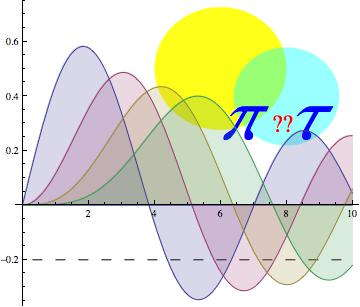
\includegraphics[width=70mm]{chapter-1/drawing.jpg}\label{subfig:drawing-jpeg}}
	\hspace{2em} % Inserts space between subfloats on the same line.
	\subfloat[PNG version.  If you must use a bitmap format, prefer PNG to JPEG.]{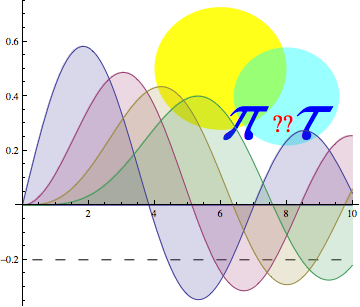
\includegraphics[width=70mm]{chapter-1/drawing.png}\label{subfig:drawing-png}}
	\\ % Additional subfloats will be on a new line.
	\subfloat[PDF version.  Obviously better than the other formats for generated graphics.]{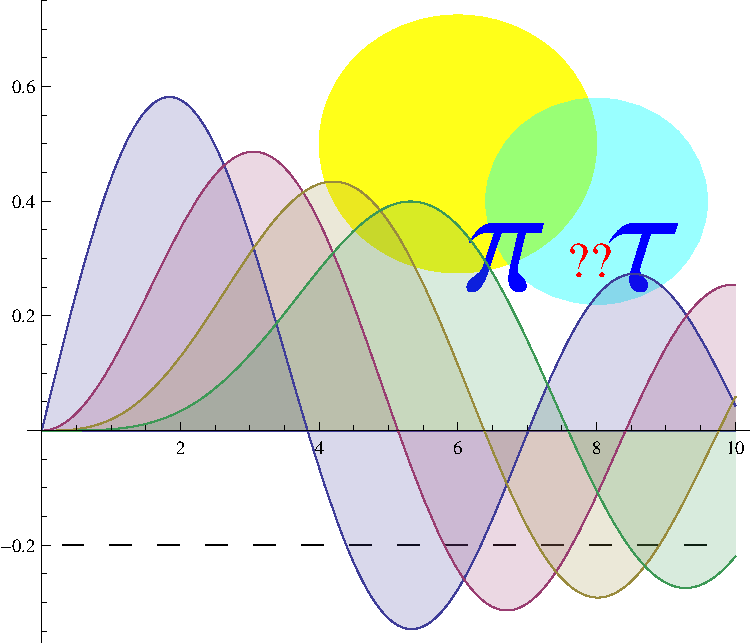
\includegraphics[width=70mm]{chapter-1/drawing.pdf}\label{subfig:drawing-pdf}}

	\label{fig:drawing}
\end{figure}

\section{Lists in \texttt{thesis} class}

In \texttt{thesis} class (for Colorado University), lists are defined so that
nested lists will be numbered or marked appropriately.  First, an itemized
(non-enumerated) list prefaces each item with a bullet.  Nested itemized list
use asterisks, then dashes, then dots.  These lists are typed between the
\verb2\begin{itemize}2 and \verb2\end{itemize}2 commands.

\begin{itemize}
  \item{} This is ``itemized'' item A.
  \item{} This is ``itemized'' item B.
  \item{} This is ``itemized'' item C.
  \begin{itemize}
    \item{} This is ``itemized'' subitem A.
    \begin{itemize}
      \item{} This is ``itemized'' subsubitem A.
      \begin{itemize}
        \item{} This is ``itemized'' subsubsubitem A.
      \end{itemize}
      \item{} This is ``itemized'' subsubitem B.
    \end{itemize}
    \item{} This is ``itemized'' subitem B.
  \end{itemize}
  \item{} This is ``itemized'' item D.
\end{itemize}

Enumerated lists use the commands \verb2\begin{enumerate}2 and
\verb2\end{enumerate}2, and nested enumerations appear like this.

\begin{enumerate}
  \item{} This is ``enumerated'' item A.
  \item{} This is ``enumerated'' item B.
  \item{} This is ``enumerated'' item C.
  \begin{enumerate}
    \item{} This is ``enumerated'' subitem A.
    \begin{enumerate}
      \item{} This is ``enumerated'' subsubitem A.
      \begin{enumerate}
        \item{} This is ``enumerated'' subsubsubitem A.
      \end{enumerate}
      \item{} This is ``enumerated'' subsubitem B.
    \end{enumerate}
    \item{} This is ``enumerated'' subitem B.
  \end{enumerate}
  \item{} This is ``enumerated'' item D.
\end{enumerate}

\begin{table}[htb]
  \caption[Example of a table with its own footnotes]{
		Here is an example of a table with its own footnotes.  Don't use the
		\texttt{$\backslash$footnote} macro if you don't want the footnotes at the
		bottom of the page.  Also, note that in a thesis the caption goes
		\emph{above} a table, unlike figures.  (Well, so the original version of the document said---but my thesis showed captions under the tables.)
		\\
		You should try using the \texttt{tabularx} command, instead of just \texttt{tabular}.  In addition, check out the \href{https://ctan.math.utah.edu/ctan/tex-archive/macros/latex/contrib/booktabs/booktabs.pdf}{documentation} for \texttt{booktabs}.
		\\
		Note there are no vertical lines in this table and few horizontal lines, too.  Plus, we've stretched the table to be the full text width, which is how Physical Review does it.  Much nicer.
	}

	% Using the "X" column type makes LaTeX decide on the column width for you
	% while stretching the table to the desired width (\textwidth, in this case).
	%
	% You can also use the new L, C, and R column types (defined in the preamble)
	% for left, center, and right aligned paragraph-formatted table columns.
	\begin{tabularx}{\textwidth}{XXXXX}
	\toprule
	& $S$ & $P$ &   $Q^{\ast}$  & $D^{\dagger}$ \\	% footnote symbols!
	Wave form & (kVA) & (kW) & (kVAr) & (kVAd) \\
	\midrule
	\cref{subfig:drawing-jpeg}  & 25.48 & 25.00 & -2.82 & 4.03 \\
	\cref{subfig:drawing-pdf}  & 25.11 & 18.02 & -9.75 & 14.52 \\
	\cref{tab:pdftable}  & 24.98 & 22.26 & 9.19 & 6.64 \\
	\cref{tab:powertable}  & 23.48 & 15.00 & 6.59 & 16.82 \\
	\cref{fig:pyramid}  & 24.64 & 22.81 & -0.44 & 9.3 \\
	\bottomrule
	\end{tabularx}

	% Apparently you can shove arbitrary text here and LaTeX will just render it.
	% Us these for these footnotes.
	\begin{center}
		${}^\ast$kVAr means reactive power. \\
		${}^\dagger$kVAd means distortion power.
	\end{center}

	\label{tab:powertable}
\end{table}
